%%% whitepaper.tex: -*- LaTeX -*-  The general structure for the whitepaper.
%%% 
%%% Copyright (c) 2017 Brian J. Fox & Orchid Labs, Inc.
%%% Author: Brian J. Fox (bfox@meshlabs.org) Tue Oct 10 11:36:56 2017.
%%% Author: A shitload of others.
\documentclass{article}

\usepackage[utf8]{inputenc}
\usepackage[]{algorithm2e}
\usepackage{graphicx}
\usepackage{amsmath}
\graphicspath{ {images/} }
\usepackage{svg}
\usepackage[letterpaper, portrait, margin=1in]{geometry}
\usepackage{multicol}
\setlength{\columnsep}{1cm}
\usepackage[english]{babel}
\usepackage{csquotes}
\usepackage{mfirstuc}

\usepackage[backend=biber,style=numeric-comp,url=true]{biblatex}
\bibliography{whitepaper}

%% \addtocontents{toc}{\protect\setcounter{tocdepth}{0}}
\newcommand{\orchid}{Orchid}
\newcommand{\Orchid}{\orchid}

\usepackage{titlesec}
\titlelabel{\thetitle.\quad}

\title{\Orchid: A Fully Distributed, Anonymous Proxy Network Incentivized Through Bandwidth Mining}
%%% draft.tex: -*- LaTeX -*-  DESCRIPTIVE TEXT.
%%% 
%%% Copyright (c) 2017 Brian J. Fox
%%% Author: Brian J. Fox (bfox@opuslogica.com) Sun Oct  8 07:14:09 2017.
\usepackage{draftwatermark}
\SetWatermarkText{INTERNAL DRAFT}
\SetWatermarkScale{2}

\title{\Orchid{}: A Fully Distributed, Anonymous Proxy Network Incentivized Through Bandwidth Mining \\ (INTERNAL DRAFT - NOT FOR DISTRIBUTION)}

\author{{David L. Salamon with} \\ {Jay Freeman, Gustav Simonsson, Brian J. Fox} \\ {{Stephen F. Bell, and Dr. Steven Waterhouse, Ph.D.}}}
\date{\today{}}

\raggedbottom

\begin{document}

\maketitle

\begin{abstract}
%%% abstract.tex: -*- LaTeX -*-  DESCRIPTIVE TEXT.
%%% 
%%% Copyright (c) 2017 Brian J. Fox & Orchid Labs, Inc.
%%% Author: Brian J. Fox (bfox@meshlabs.org) Tue Oct 10 11:36:56 2017.
%%% Author: A shitload of others.
  As methods for censoring browsing and discovering private browsing information have improved, interest in anonymization methods has increased. Unfortunately, existing approaches to unrestricted, unsurveilled Internet access such
as I2P and Tor suffer from a tragedy of the commons – only a few thousand unpaid volunteers host proxies and exit nodes, allowing sophisticated attackers a tractable number of nodes to monitor or otherwise compromise. We present a market based, fully decentralized, anonymous peer-to-peer system based on “bandwidth mining” which we hope will address this lack of relays by paying them.

  %% The Internet's current structure is the product of two forces: (1)
  %% what is easy to implement for a small to medium sized company, and
  %% (2) the desires of mankind.

  %% Unfortunately, not all desires of mankind have proved agreeable. For
  %% example, as methods for censoring browsing and discovering private
  %% browsing information have improved, consumers have found themselves
  %% in the unenviable position of needing to decide between their
  %% privacy and usable Internet access. Even for those willing to suffer
  %% the usability hit, current methods to achieve unrestricted,
  %% unsurveilled Internet access such as I2P and Tor suffer from a
  %% tragedy of the commons – only a few thousand unpaid volunteers host
  %% proxies and exit nodes, allowing sophisticated attackers a tractable
  %% number of nodes to monitor or otherwise compromise.

  %% Similarly, not all desirable services have proved easy to
  %% implement. Perverse economic incentives stemming from widely
  %% available free content have resulted in a news media bereft of
  %% subscribers, slowly descending into a minute-to-minute battle for
  %% clicks. The high cost of distributing video has resulted in
  %% centralization, platforms, and burdens on content creators. The
  %% difficulty of maintaining and securing a sever have resulted in less
  %% diversity than one might have hoped for.

  %% To address these issues, we present a high performance approach to
  %% networking built on a foundation of micropayments, and as an initial
  %% application of the technology, build an uncensorable, anonymous
  %% mechanism for accessing the global Internet. It is our hope that as
  %% the tokens gain in acceptance, many millions of websites will
  %% incorporate the payment models described here, and consumers will
  %% receive a monthly budget of tokens from their ISP.

  Contributions include:

  \begin{itemize}
  \item A blockchain-based stochastic payment mechanism with
    transaction costs on the order of a packet.
  \item A commodity specification for the sale of bandwidth.
  \item A method for distributed inductive proofs in peer-to-peer
    systems which make Eclipse attacks arbitrarily difficult.
  \item An efficient security-hardened auction mechanism suited for
    the sale of bandwidth in circumstances where an attacker may alter
    their bid as part of an attack.
  \item A fully distributed anonymous bandwidth market.
  \end{itemize}

\end{abstract}


\newpage
\tableofcontents
\newpage

\section{Introduction}
\label{sec:overview}
%%% introduction.tex: -*- LaTeX -*-  DESCRIPTIVE TEXT.
%%%
%%% Copyright (c) 2017 Brian J. Fox & Orchid Labs, Inc.
%%% Author: Brian J. Fox (bfox@meshlabs.org)
%%% Author: A truckload of others
%%% Birthdate: Tue Oct 10 11:59:37 2017.

\subsection{System Goals}

The \Orchid{} Network was designed with three goals:

\begin{enumerate}
\item To codify the right to unrestricted, unsurveilled Internet access on a network level.
\item To build a system suited for daily use. To say that a freedom is not a part of daily life is to say that the freedom is dying.
\item To make such a system worthy of trust, by developing it in the open and releasing the source code for full public audit.
\end{enumerate}

These are ambitious goals, and are not realized by the system described in this document. This document does, however, contain an imperfect first attempt – an invitation to join us in design, construction, and use of what we believe is the future of networking.

\subsection{Acknowledgements}

We would like to extend special thanks to Professor Dan Boneh, Professor Paul Vigna, Justin Sheek, Brian Vohaska, and all of our early investors and advisors. Without their passion for this problem domain, and their willingness to take a risk chasing a solution, this project would not have seen the light of day.

\subsection{Terms}

\begin{itemize}
\item Node. A computer running a program which implements the \Orchid{} Protocol.
\item Medallion. Data used by a node to demonstrate it is in exclusive possession of computational resources.
\item User. The owner of a node.
\item Orchid Market. A P2P collection of nodes interacting through the \Orchid{} Distributed Marketplace Protocol.
\item \emph{The} Orchid Market. \TOM{} in possesion of the most global computational power.
\item Customer. A buyer on \tOM{}.
\item Peddler. A node who is a member of an Orchid Market's collection.
\item Entry Peddler. A Peddler who is willing to accept direct TCP connections from Customers.
\item Address. The location in Medallion-space inhabited by a Peddler.
\item Relay. A Peddler willing to sell bandwidth to customers.
\item Proxy. A Relay which is additionally willing to interact with web servers on behalf of Customers.
\item Chain. A list of n Relays ending in a Proxy used for anonymous communication by a Customer.
\item Ticket. A stochastic micropayment.
\item Attack. A method for causing the non-consensual transfer of money or information.
\item Attacker. A person or group of people interested in performing attacks.
\end{itemize}

\subsection{High-Level System Overview}

\subsubsection{\TOM{}}

\begin{figure}[htbp]
  \centering
  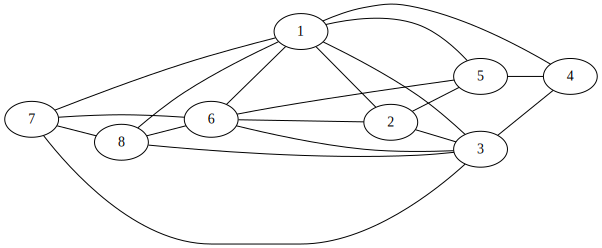
\includegraphics[width = 300pt]{marketOverview}
  \caption{An Orchid Market with eight Peddlers}
\end{figure}

\TOM{} is a globally distributed P2P market place for bandwidth. \TOM{} connects Peddlers to each other randomly, and has each Peddler verify the ``realness'' of its connected peers.

\subsubsection{Chains}

\begin{figure}[htbp]
  \centering
  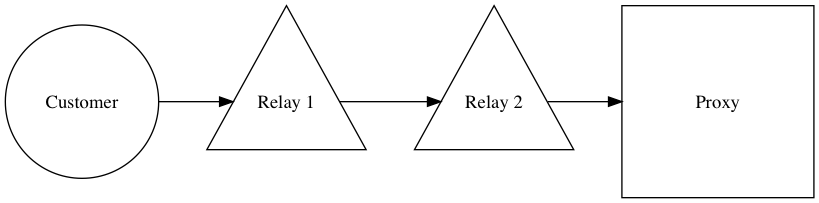
\includegraphics[width = 300pt]{sttc}
  \caption{A three-Peddler Chain routing traffic for a Customer}
\end{figure}

Once relay and proxy bandwidth has been purchased, the customer configures them into a directed acyclic graph termed a Chain. In the above picture, Relay 1 receives bandwidth from the Customer, performs cryptographic operations on it, and forwards the resulting data to Relay 2. Relay 2 performs a similar role with respect to Relay 1 and the Proxy. The Proxy then sends this data to a web server. Any data returned by the web server is sent back to the Customer along another chain, perhaps implemented using the same nodes in reverse.

\subsubsection{Web Browsing}

The majority of initial usage of the \Orchid{} Network will likely happen in support of uncensorable, anonymous web browsing. In this use case, the client software will automatically use \tOM{} to create a Chain, and provide additional checks to verify that SSL/TLS is being used in a way suited to this networking model. Unless two or more nodes in a Chain are working together (Section \ref{sec:collusion}), perhaps because they are run by the same user, no single node knows the Customer's IP Address and the server they communicated with.

\subsection{User Stories}

\subsubsection{Bandwidth Miners}

Users with excess computational power and bandwidth may choose to support the \Orchid{} Network, as well as earn money, by running a Peddler on their computer. To do so, they install and run the \Orchid{} software package and supply a payment address. To verify realness while preserving anonymity, the software will convert computational resources into Medallions. Peddlers are compensated for their lost computation by bandwidth consumers.

\subsubsection{Resisting Oppressive Governments}

Users who live under oppressive regimes (where, for example, it is illegal to access Wikipedia), can use the system to hide information about the websites they are browsing. To do so they install and run the \Orchid{} software, provide an initial payment to their \Orchid{} wallet, and browse the web as normal. Unlike similar services (Section \ref{sec:prior-work}), the network pays hosts for their participation. We hope this will lead to greater participation, which in turn will lead to grater anonymity (Section \ref{sec:market}).

\subsubsection{Resisting Oppressive Web Applications}

Users of oppressive web applications (sites which change services offered based on geographic location), can use the \Orchid{} Network to appear to be browsing from the country of their choice. Unlike similar services (Section \ref{sec:prior-work}), traffic will not come from IP ranges allocated to server farms, and so will be much harder for oppressive websites to block. Additionally, because bandwidth is incentivized, it will likely prove much more plentiful on the \Orchid{} Network, i.e. making the real-time playback of high resolution video viable.


\section{Attacks}
\label{sec:attacks}
%%% attacks.tex: -*- LaTeX -*-  DESCRIPTIVE TEXT.
%%%
%%% Copyright (c) 2017 Brian J. Fox & Orchid Labs, Inc.
%%% Author: Brian J. Fox (bfox@meshlabs.org)
%%% Author: A truckload of others
%%% Birthdate: Tue Oct 10 12:00:13 2017.

As much of this paper is on attack prevention, we begin by reviewing
the literature on those attacks which are particularly common against
P2P networks.

\subsection{Attacker Goals}

\subsubsection{Information Gathering}

The largest class of attacks against which the \Orchid{} Protocol must defend against are those which reveal information about its users. Because \Orchid{} is implemented as an overlay on the existing Internet, some information is \emph{unavoidably} shared with some peers. In the list below, such information is marked with a “*”. Any information which is not specifically listed as \emph{unavoidably} shared in this document, but for which a method is discovered to uncover that information is termed an \emph{informational attack} and is covered by \Orchid’s White Hat Bug Bounty. For more information on what is shared, see the protocol specification in Section \ref{sec:mining} and discussion of collusion in Section \ref{sec:collusion}, and our reference implementation of the network\cite{oursoftware}.

Types of data which are assumed to be of interest to an attacker (timeless):

\begin{itemize}
\item Real-World Identity Information. A user’s given name, SSN, address, etc.
\item Website Account Information. The user accounts at a specific website. Note this can be different from Real-World Identity Information.
\item *IP Information. The IP address from which a user is accessing the \Orchid{} Network. Note that in some usage scenarios this may be equivalent to learning Real-World Identity Information.
\item *Ethereum Information. The keys associated with a user’s wallet (*public or private). Note that in some usage scenarios this may be equivalent to learning Real-World Identity Information.
\item *\Orchid{} Network Information. The keys associated with a node’s current business on the \Orchid{} network (*public or private).
\end{itemize}

Types of Behavioral information which are assumed to be of interest to an attacker (time and Chain associated data):

\begin{itemize}
\item *Customer Identification. The attacker learns the IP address of a customer.
\item *Relay Identification. The attacker learns the IP address of a relay.
\item *Proxy Identification. The attacker learns the IP address of a proxy.
\item *Link Identification. The attacker learns that two IP addresses were employed in a Chain.
\item *Website Access. The attacker learns that an outbound connection was made from the \Orchid{} network to a specific website.
\item *Webserver Access. The attacker learns that an outbound connection was made from the \Orchid{} network to a specific webserver (which may host multiple websites).
\item *Ethereum Linking. The attacker learns that an Ethereum public key is held by a \Orchid{} user.
\item *Purchase Linking. The attacker learns that two transactions share a common payer.
\item *Purchase Information. The attacker learns the quantity and timing of bandwidth sent over a Chain.
\end{itemize}

Although all of the above behavioral information is shared with other nodes on the \Orchid{} Network during normal operation, as described below, in most contexts it is assumed that users will only be directly harmed by \textbf{Behavioral Information Gathering} if the attacker can learn several pieces of information at once. For example, to say that user X accessed website Y the attacker would need: buyer identification, website access information and several pieces of link identification. For this reason, peers following the reference specification do not store or share any of the above information except as required to provide the services a customer has purchased.

\subsection{Economic Attacks}
\label{econ-attacks}

Unlike similar systems, \Orchid{} Network must also concern itself with attacks on payment mechanisms. The taxonomy used in this paper is:

\begin{enumerate}
\item \textbf{Economic Exploits}. Profitable undesirable behavior such as a user providing “free sample” bandwidth allowing users to exclusively use free sample bandwidth.
\item \textbf{Economic Denial of Service (EDoS)}. Using payments to overwhelm another node on the \Orchid{} Network with purchases, thereby taking them offline.
\end{enumerate}

\subsection{Quality of Service Attacks}
\label{qos}

Some adversaries may be satisfied by slowing down system performance of \Orchid{} Network users generally, thereby potentially diminishing usage.

\subsection{Man-in-the-Middle Attacks}
\label{mitm}

Actions that can be performed only after inserting oneself between two interacting parties are collectively referred to as man-in-the-middle attacks. Encrypted information may be logged for analysis of metadata (Section \ref{inference-attacks}), while non-encrypted data may additionally be changed to control behavior. If key exchange is not secured, the man-in-the-middle may also trick two parties into wrongly believing the attacker's key is the other party's key.

\subsection{Sybil Attacks}

Malicious actions, performed by pretending to be multiple users, are termed Sybil Attacks, after a patient suffering from multiple personality disorder. Applications of this type of attack include:

\begin{itemize}
\item Submitting multiple reviews to Yelp, Amazon, etc.
\item Achieving faster downloads on BitTorrent by pretending to be multiple leachers\cite{freeridingBittorrent}.
\end{itemize}

\subsection{Eclipse Attacks}

In an Eclipse Attack, the attacker's goal is to hide part of a system from itself. The methods employed are generally the network equivalent of privilege escalation attacks: gain control of network positions which have more control of the network, then use that control to acquire more control.

\begin{itemize}
\item Segmenting the Bitcoin mining P2P network, allowing for so-called “51\% attacks” when the attacker controls substantially less than 51\% of the compute power\cite{bitcoinEclipse}.
\item Removing a file from the BitTorrent DHT by taking over the address space associated with its magnet link\cite{bittorrentSybilAttacks}.
\end{itemize}

\subsection{Denial of Service Attacks}

Attacks centered around taking a specific resource offline are termed Denial of Service Attacks (DoS). System behavior during “unexpected” circumstances is often poorly specified and tested. DoS attacks are useful for deanonymizing nodes in P2P networks. Notable examples:

\begin{itemize}
\item Targeted DoS attacks used in concert with Sybil Attack based monitoring to deanonymize Tor traffic\cite{DOSvsSec}.
\item DoS off-lining for complete control of I2P’s floodfill database, requiring only 20 Sybil nodes, thereby deanonyimizing all traffic on the network\cite{I2P-vigna}.
\end{itemize}

\subsection{Inference Attacks}
\label{inference-attacks}

Deanonymization which stems from statistical modeling system behavior are termed Inference Attacks or Monitoring Attacks. These are often combined with “probing moves” such as carefully crafted or timed requests, or other attacks such as DoS-ing a specific peer off of the network and observing how traffic patterns respond.

\begin{itemize}
\item Inferring medical illnesses, family income, and investment choices of end-users from SSL encrypted web traffic\cite{broadInferenceAttacks}.
\item Deanonymizing Tor, I2P and \Orchid{} traffic from global traffic logs\cite{mixTrafficAnalysis}.
\item Learning the private key of an OpenSSL server through timing analysis\cite{opensslTimingAttack}.
\end{itemize}

\subsection{Hacking}

By converting historically trustworthy peers into attack vectors, motivated attackers might directly compromise nodes on the network. When bandwidth is deployed using Chains, iterative hacking may eventually allow an attacker to ``backtrace'' a connection. Such attacks have important security implications but are out of the scope of the \Orchid{} Network. If the \Orchid{} Network's design achieves its goals, this will be the main attack against users of the system.


\section{Alternative Approaches}
\label{sec:prior-work}
%%% approaches.tex: -*- LaTeX -*-  DESCRIPTIVE TEXT.
%%%
%%% Copyright (c) 2017 Brian J. Fox & Orchid Labs, Inc.
%%% Author: Brian J. Fox (bfox@meshlabs.org)
%%% Author: A truckload of others
%%% Birthdate: Tue Oct 10 12:01:02 2017.

\subsection*{Unprotected Internet Access}

Users who access the Internet without protection provide their
complete browsing history and website use to their ISP, who can then share or sell that data.

\subsection*{Virtual Private Networking (VPN) Services}

Virtual Private Networks (VPNs) use encryption to securely transport a
VPN subscriber's traffic across a larger insecure network. Once the
VPN has received the traffic, it is decrypted and retransmitted across
a different large insecure network. The retransmission can assist
users in circumventing access restrictions imposed by websites, and to
a lesser extent, reduce the tracking of their website browsing
habits. Encryption prevents the user's ISP from seeing their traffic,
thereby preventing monitoring attacks. This is accomplished by making
the VPN a new ISP for the user.  Any attack an ISP could previously
perform can easily be performed by the VPN provider.

VPN users should not assume their VPN provider is trustworthy. Although VPN service providers face more competition
than ISPs, they ultimately draw talent from the same sources, and have
similar bandwidth-for-cash-type business models. It is unlikely that
VPN providers will not fall prey to the same incentives which led the
user to not trust their ISP. Additionally, the re-use of IP addresses
for relaying traffic in VPN setups enables relative ease in blocking
their use by commercial websites\cite{13}.

\subsection*{Tor}

Tor\cite{TOR} is a free software project famous for introducing the
idea of \emph{Onion Routing} to a wider audience. In this system, users
download a global list of relays and exit nodes, randomly select from
that list, and form \emph{onion routes} from their selection. Onion
routes are an ordered list of relays; packets sent along an onion
route are encrypted for each peer in turn, ensuring that each node
must have received a packet enroute for it to be understood by the
exit node. The result is that unless several nodes are compromised or
run by the same user, no two relays know both who sent 
a packet and where it went.

\begin{figure}[htpb]
  \centering
  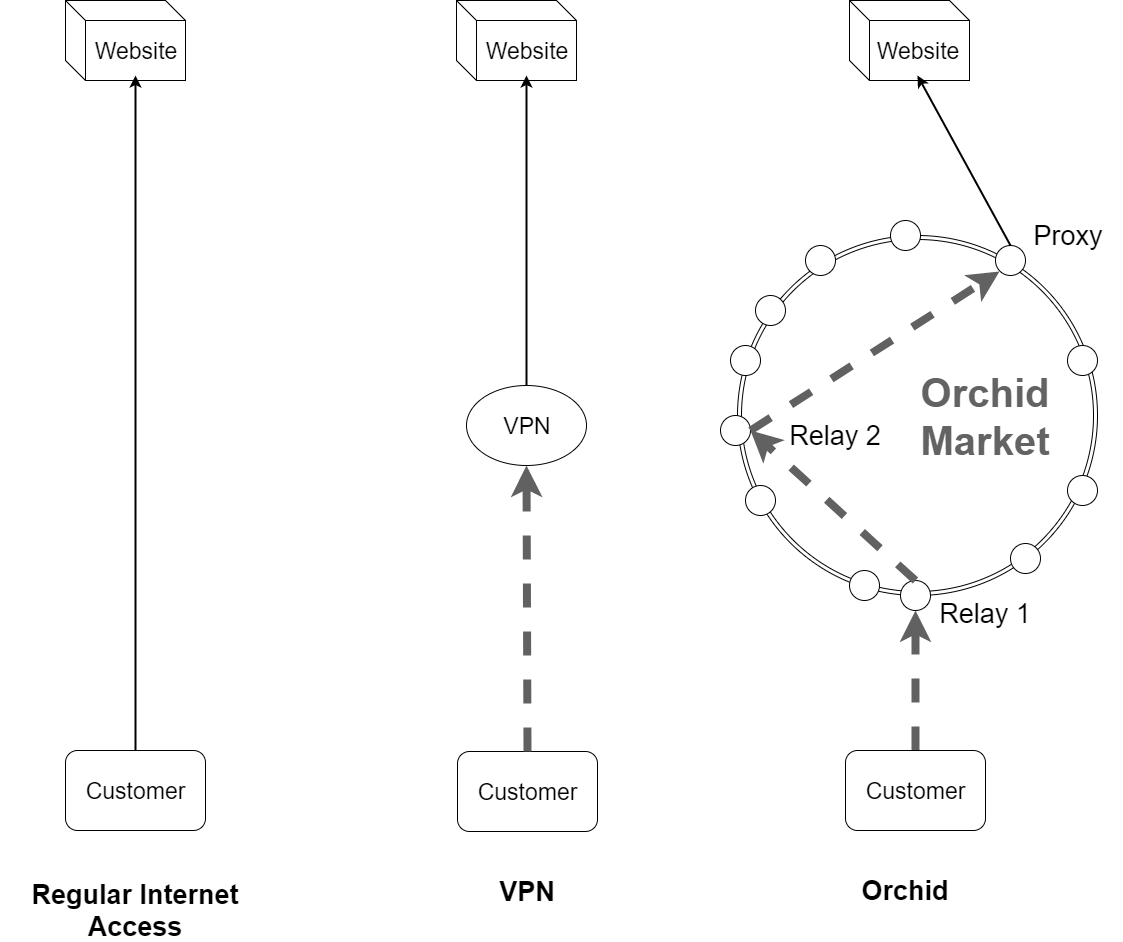
\includegraphics[width = 400pt]{overview}
  \caption{Direct connection, VPN connection, Orchid connection}
\end{figure}

%% @saurik: ref on Dingledine knowing ~75% of relay operators personally?

%% \subsection{Tor with Incentives} ?

%% \subsection{I2P} ?

%% I2P is billed as a “next generation” onion router. It is primarily
%% focused on communication internal to the network.

%% \subsection{Mixmaster, Mixminion, and other Chaumian relay schemes} ?


\section{External Libraries}
\label{sec:external-libraries}
%%% external-libraries.tex: -*- LaTeX -*-  DESCRIPTIVE TEXT.
%%% 
%%% Copyright (c) 2017 Brian J. Fox & Orchid Labs, Inc.
%%% Author: Brian J. Fox (bfox@meshlabs.org)
%%% Author: A truckload of others
%%% Birthdate: Tue Oct 10 12:01:48 2017.

\Orchid’s functionality is built on several important primitives. As some readers may not be familiar with these primitives, or be familiar with the specific properties used in the \Orchid{} Network, we briefly summarize them here.

\subsection{WebRTC}

WebRTC\cite{webrtc} is a system originally designed to facilitate real-time communication between web browsers. It provides excellent implementations NAT and firewall traversal methods, including STUN, ICE, TURN, and RTP-over-TCP. By selecting WebRTC as the basis for our networking protocol, rather than custom coded TCP and UDP networking code, we both get a world-class implementation of these technologies, and (to an extent) mask our user's traffic as general web traffic.

\subsection{NACL}

NaCL\cite{nacl} is a cryptography library by Daniel J. Bernstein et al., focused on building the core operations needed to build high-level cryptographic tools. It was chosen as the source for cryptographic primitives on this project due to both it and its author's sterling reputation. All cryptographic operations described below are implemented using NaCL, aside from Ethereum smart contract cryptographic code.

\subsection{Ethereum}

Ethereum\cite{ethereum} is a decentralized blockchain and platform that includes a native currency (ETH) and Turing-complete smart contracts. The smart contracts proved extremely useful for the design of \Orchid, allowing us to offload a plethora of design concerns related to the tracking of token balances and the verification / fairness of our \emph{Ticket} payment channels.



\section{Medallions}
\label{medallions}
%%% medallions.tex: -*- LaTeX -*-  DESCRIPTIVE TEXT.
%%%
%%% Copyright (c) 2017 Brian J. Fox & Orchid Labs, Inc.
%%% Author: Brian J. Fox (bfox@meshlabs.org)
%%% Author: A truckload of others
%%% Birthdate: Tue Oct 10 12:02:20 2017.

Fully decentralized, fully anonymous digital systems suffer from attacks in which a single malicious user pretends to be thousands of users (Sybil Attacks) {\color{red}[REFERENCES]}. To mitigate the generation of Sybils and other effects of this class of attack, the \Orchid{} Protocol employs a proof-of-work scheme. We call the tokens of this scheme Medallions. Each Medallion contains data that cryptographically demonstrates the generator possessed a \textit{sizable} computation resource at a given time. As
computation is an expensive resource, the use of Medallions places budgetary limitations on a given attacker's ability to impersonate multiple users.

\subsection{Medallion Proof-of-Work}
\label{medallion-pow}

Medallions form the bridge between our core security assumptions and the network as a whole. Since our fundamental security goal is to limit a well-motivate attacker from gaining control of the \Orchid{} Network, our choice of Medallion creation must meet the following conditions,
  \begin{enumerate}
      \item Medallion creation must be \textit{easy} for a non-malicious node to create
      \item Medallions  must be \textit{easy} to verify
      \item Medallions must be \textit{difficult} to create in bulk
  \end{enumerate}
With these conditions, we define \textit{difficulty} to mean prohibitive scalability in time and money. In short, we want a proof-of-work system where it is \textit{easy} for a normal node to obtain entry to the network but difficult for an attacker to scale entry into the network. In {\color{red}[SECTION]} we discuss our choice of proof-of-work over other methods such as proof-of-stake \cite{bentov2016snow, kiayias2017ouroboros, houy2014will} and proof-of-space \cite{dziembowski2015proofs, park2015spacecoin}.

Two primary methods currently exist that satisfy the requirements above: challenge-response protocols, and crypto-puzzles. Unfortunately, challenge-response protocols may not provide sufficient security within the Orchid model as an attacker may be able to precompute challenge and responses via collusion. This leaves crypto-puzzles of which there are many in existence today \cite{nakamoto2008bitcoin, Equihash} each with their own trade-offs. Again, in order to satisfy the requirements of Orchid only a subset of those crypto-puzzles are suitable. Namely, crypto-puzzles which can not easily be parallelized, made into an ASIC, or scaled trivially. Recently, researchers have discovered algorithms that produce easy-to-verify results that have tunable creation difficulty \cite{Equihash}. These collection of algorithms exploit the trend that memory and total silicon area is expensive to scale \cite{abadi2005moderately, dwork2005pebbling}. These class of algorithms are called asymmetric memory-hard functions and we use them for medallion creation. There are several varieties of these functions \cite{tromp2014cuckoo, lorimermomentum, Equihash} but we have chosen to use Equihash. Equihash is based on the k-XOR birthday problem and provides memory hardness via a time-space trade-off\footnote{It is no coincidence that this time-space trade-off is reminiscent of time-memory trade-offs as first discovered by \cite{hellman1980cryptanalytic}}. Since Equihash is tunable, simple, is based of an NP problem, and has gained acceptance in the cryptocurrency community, we believe that using such a function as our basis for proof-of-work provides an acceptable level of security and future-proofing.

To produce a medallion, a peer takes a public key $K$, and the previous Ethereum block hash $E$, then performs a series of computations in order to locate a salt $S$ such that $\mathcal{F}(K, E, S, ...) \geq N$, where $N$ is some difficulty scaling factor. When a new Ethereum block is added to the chain, a new $S$ must be calculated to keep the Medallion current. The Medallion specification will be discussed in {\color{red}[SECTION]}.

\subsection{Selection of Proof-Type}
\label{medallion-proof}

Readers familiar with other market-based distributed networks will recognize that our use of Medallions is similar in premise to other proof-of-work systems (bitcoin, etc). Further readers may be inclined to ask: why not use proof-of-stake, proof-of-idle, or other methods for earning acceptance into the \Orchid{} Protocol and specifically \tOM{}? In this section we describe why we have chosen proof-of-work over other methods.

\subsubsection{Proof-of-stake}

{\color{red}[DEFINE proof-of-stake]}. Proof-of-stake
rests on the assumption that no attacker will ever control the majority of tokens {\color{red}[REFERENCE]}. {\color{red}[State Attack]}. As our attack model includes governments that are well-motivated, well-resourced, and possibly oppressive, proof-of-stake assumption can not be counted as always being true. Even Bitcoin’s astonishing market capitalization is far less than the GDP of a modestly sized country. {\color{red} [Example attack using bitcoin]} Making matters more complicated, in the near future we intend to extend the system to support anonymous payments, which will make detection of such a ``hostile takeover'' much more difficult. Thus, we could not base Medallions on a proof-of-stake model as sufficient stake in the system could permanently and irreversibly compromise the anonymity and security of the \Orchid{} Protocol. In short: we did not use proof-of-stake because we did not want to engineer a system in which our users’ right to privacy might be sold to the highest bidder.

\subsubsection{Proof-of-space}
%%%%% This section needs more work--we may have said things that might not be true %%%%%%%

In a proof-of-space, computational resources like those used in proof-of-work systems are traded for storage space. In short, proof-of-space is an \textit{interactive} protocol where two participants--a prover and a verifier--interact to verify that the prover has some amount of storage space by performing verifier-guided calculations. The assumption is that these calculations would only be practical if the prover stored and recalled them\cite{dziembowski2015proofs}. Although we are not sure that a suitable method will be located, we are exploring the possibility of using proof-of-space for an upcoming version of the \Orchid{} Protocol. This would allow old smart phones 
{\color{red}[<--I don't this this is true; P-o-S uses large cryptographic super-concentrators w/ GB->TB of space; this is referenced in the equihash paper. I think equihash would prob work just as well if the super-concentrator isn't HW accelerated. In particular, Id be worried about performance. The PoS paper doesn't mention performance at all and states that it used graph traversal in order to accomplish its goal; since no performance or security data is given we don't know how big the graphs need to be, how much CPU is required to build them, the storage IO time needed to store them, recall time, SSD/RAM/HDD differences, or security/usability implications to each of these choices.]}
, for example, to be installed by users in their homes as Relays and Proxies. For more on this idea, see Section \ref{future:proof-of-space}. {\color{red}[That section says the same thing as the text here]}

\subsubsection{Proof-of-idle}

{\color{red}[DEFINE proof-of-idle]} Proof-of-idle rests on the additional assumption that periodic, synchronized proof-of-work is sufficient to demonstrate a User’s share of the global computational power. Unfortunately, while the network is in its infancy ($\leq$ 10 million Peddlers), this leads to a situation where any company in control of a supercomputing center may, with only the sacrifice of ~1\% of their computational power, take control of the network. As we expect it to be quite a while before we have sufficient numbers of Peddlers for this attack to cease being devastating, we are not using proof-of-idle for this release.

\subsection{Medallion Specification}
\label{medallion-spec}

At a high-level, generating a Medallion involves two steps, (1) generation of a public/private key pair $K$ and retrieval of the most recent Ethereum block digest $E$ and (2) (iteratively or in parallel) locating a salt $S$ such that $\mathcal{F}_{N}(K, E, S)$ wins for some winning condition where $N$ is some difficulty scaling factor. Recall that the goal of the Medallion is to provide proof-of-work for a specific entity. Thus each Medallion must be cryptographically linked to a specific public key so that no Medallion can be used to impersonate multiple peers. Moreover, we want to limit the amount of precomputation advantage that any entity could leverage. Hence, Medallions are cryptographically tied to an Ethereum block digest which changes on the order of 10s of seconds. The following are definitions for the Medallion specification,

\begin{enumerate}
	\item[] $pk_m$ is a unique public key belonging to a peer$_m$
    \item[] $sk_m$ is a unique secret key associated with $pk_m$
    \item[] $e_t$ is the Etherium block digest at time $t$ 
    \item[] $h(y)$ is the digest of a cryptographic hash function with input $y$
    \item[] $sig(sk, r)$ is the basic signature of $r$ using secret key $sk$
    \item[] $\mathcal{F}_{n,k}(x_j)$ is Equihash output\footnote{Note that the output of $\mathcal{F}(x_j)$ is a set of counters $j$ such that for XOR$_j=h(j)$, $\sum$XOR$_j$=0 for all j in the output.} with starting counter $x_j$ and difficulty $(n,k)$
    \item[] $seed$ is $h(e_t|sig(sk,e_t))$
\end{enumerate}

$h(y)$ could be any cryptographic hash function but the \Orchid{} protocol uses {\color{red} [KECCACK]}. A discussion of this hash function choice can be found in {\color{red}[SECTION]}. We define a basic signature to be the exponentiation of appropriately sized some data by a secret key. 

Using these definitions we define a Medallion to be the set,
						$$\mathcal{M} = \{t, e_t, pk_m, sig(sk,e_t), \mathcal{F}_{n,k}(seed)\}$$
for a globally agreed upon Equihash difficulty parameters $(n,k)$. For more information about these parameters see \cite{Equihash}.  Note that using $seed$ as input to $\mathcal{F}$ cryptographically links a peer's private key with the Medallion. Since Medallions determine a peer's Chord-address in \tOM{}, any entity possessing a Medallion can verified using the $pk_m$ associated with the specific peer. Moreover, an entity can ask for proof of ownership of a public key from a specific Chord-address. {\color{red}[<---this needs more explanation as to why it's important]}. Engineering details of Medallions are discussed in Appendix {\color{red}[SECTION]}. 


% If needed to explain why time-space trade-offs are important but probably a bit much:
%
%	Time-space trade-offs are an analog to time-memory trade-offs often used in cryptanalysis. These methods take 
%	advantage of intermediate computations that allow a hard problem to be more efficiently solved if some amount 
%	of pre-computation or computed state is performed. In the case of Equihash, storing k-bit strings allows one to 
%	store possible XOR wins and perform linear algebra on the system to obtain a result. Notice that this is not
%	unlike sieving in the quadratic sieve.




























\section{Tickets}
\label{sec:tickets}

Paying for bandwidth presents a rather unique set of challenges. In most other payment systems, the cost of an item is substantially greater than the cost of sending a packet, and so the networking cost may be safely ignored as just another transaction cost. In the \Orchid{} Network however, the cost of a packet is the \emph{price being paid}, and so even if the transaction costs for sending payment are as low as a single packet, they would be equal in cost to the purchased item. Making matters more troublesome, we will soon see that the transaction costs also include paying miners on the Ethereum block chain.

\subsection{How Much Will A Packet Cost?}

For the purposes of this discussion, let us assume that a packet is 1e3 bytes in length. To calculate an upper bound, we observe that the most expensive bandwidth known to mankind is AWS's Singapore CloudFront bandwidth, at \$0.14 per 1e9 bytes. This yields a per-packet cost of 1.4e-5 cents (\$0.00000014). Because bandwidth is a wasting good (any unsold bandwidth is lost forever), the actual price is likely to be significantly lower than this upper bound.

\subsection{Ethereum Transaction Costs}

Because the \Orchid{} System uses Ethereum as its payment processor, we might also be curious about what the expected cost of sending money in the system is. Although the transaction costs may vary according to [Gustav please save me]. A reasonable estimate of likely transaction costs are \$0.20 for urgent type transactions (happening on the order of 20 seconds), down to \$0.01 for non-urgent transactions (happening on the order of 20 minutes).

\subsection{Building Micropayments from Macropayments}

With transaction costs now discussed, and looming large, let us now look at what methods exist for controlling them.

One potentially interesting approach, which was employed in MojoNation\cite{mojonation}, is to have a ``balance of trade'' between each pair of nodes. As bandwidth flows between them, they periodically settle up when the balance gets too far from zero. However, as we have seen, the transaction costs of settling up using Ethereum as a payment processor in this scheme would result in at minimum a \$0.01 transaction fee. Using our upper bound, we can see this price is around 100 megabytes of bandwidth. A secondary issue with this approach, is that peers nearing the reconciliation threshold would know that fact, and be tempted to disconnect and create a new identity rather than pay the fee. For these reasons, is tempting to believe that there exists no deterministic payment scheme suited to fully anonymous bandwidth sales using Ethereum as the payment processor. We therefore turn our attention to stochastic payments.

To explore stochastic payments, let us consider a lottery ticket (hereafter simply \emph{ticket}) which has a 1e-5 chance of being worth \$1.40. How much is it worth in expectation? The answer is 1.4e-5 cents, exactly the upper bound we established for the cost of a packet. In the event that the lottery ticket is a winner, cashing in on it with urgency will cost around 14\% ($\frac{\$0.20}{\$1.4}$) in transaction costs, and with non-urgency around 0.7\% ($\frac{\$0.01}{\$1.4}$). A surprising outcome of this approach is that the effective Ethereum transaction costs may be set arbitrary low by simply multiplying the face value by some factor, and reducing the odds of winning by the same. As this approach possesses the desired properties, we have chosen it as the method of payment in the \Orchid{} Network.

\subsection{Implementation Constraints}

Now that we have located a suitable abstraction for our payments, the question becomes: how should they be implemented? The main requirements are:

\begin{itemize}
\item The method for constructing new tickets must be reusable, as otherwise transaction fees will once again be an issue.
\item Double spending must be prevented, or failing that not profitable.
\item The system must be sufficiently performant in terms of computational cost so as not to overwhelm the cost of a packet.
\end{itemize}

Of those requirements, the last element is perhaps the most troublesome. To the best of our knowledge, no method for constructing lottery tickets exist which does not depend on computation similar to that of asymmetric encryption. A modest computer can do around 1e4 such computations per second, but can easily send 1e6 packets per second when connected to high speed Internet. For this reason, although it was not sufficient for use alone, we are forced to employ a balance-of-trade approach similar to the one mentioned above. This in turn leads to a new requirement, namely ``the balance of trade must be kept sufficiently small so as to not cause an incentive to disconnect during trade''. As this is a mechanism design issue caused by an implementation reality, let us for now focus on implementation by assuming a solution exists, and defer further discussion until Section \ref{tokens-bot}.

[Better version solicited]. We now describe a design which meets the remaining two requirements. Setup phase:

\begin{enumerate}
\item Alice deposits money into an Ethereum smart contract which will control outbound payments until some time in the future ($\geq$ 1 minute from now).
\item Bob generates a random number $N$, and sends the hash $h=H(N)$ to Alice.
\end{enumerate}

Ticket production:

\begin{enumerate}
\item Alice creates the tuple $t = (timestamp, face value, odds, nonce, h)$, signs it $s = SIG(t)$, and sends the pair $(t, s)$ to Bob.
\item Bob then computes XOR($N$, $s$), and if the result is $\geq odds$, wins.
\item To redeem winners, Bob sends $(N, t, s)$ to the Ethereum smart contract managing Alice's lottery tickets along with a payment address.
\end{enumerate}

To prevent double-spending, two methods are employed. First, some portion of Alice's initial smart-contract deposit exists only to prevent double-spending. In the event of a double spend, Alice will suffer losses of 2x the double-spend amount. However, this alone is not sufficient to prevent double-spending, because Alice might decide to over-spend on a grand scale. To address this second issue, the value of winning lottery tickets begins decreasing exponentially 20 seconds after $timestamp$, thereby providing a strong incentive for winners to cash in immediately. This immediacy is then used by Bob to compute the ``wasting rate'' of Alice's smart contract balance.

Lottery ticket type payments are not novel to \Orchid. For interested readers, we recommend the extremely detailed and helpful\cite{DAM}, which includes discussion of extending tickets to support anonymous payments.

\subsection{Balance of Trade}
\label{tokens-bot}

As mentioned above, the realities of symmetric encryption performance prevent us from sending payment with every packet, and so we need a good understanding of the risks inherent in employing a ``balance of trade'' approach. We do so here in a general setting: imagine Alice and Bob wish to transact in a fully anonymous manner. Bob is to perform some task for which he charges $x$, and Alice is to pay him once every $y$ tasks. Unfortunately, the nature of anonymity is such that without prior transactions, Alice and Bob have no mechanism to trust one another. Can they cooperate?

If there is some setup cost to Alice and Bob's relationship ($S_{Alice}, S_{Bob}$ s.t. $S_{Alice} > xy, S_{Bob} > xy$), the answer is yes: running away with the money or work ceases to be economically rational, unless (1) the total amount of work Alice was seeking was $\leq xy$ or (2) the total amount of work that Bob can perform is $\leq xy$. As we will see in our discussion of the Agora (Section \ref{sec:agora}), setup costs exist on the \Orchid{} Network which support trade imbalances in excess of 1e3 packets. Because sellers in the Agora generally pay a higher setup cost than buyers, and because Customers asymmetrically know how much work they will require, the \Orchid{} Network has Customers pre-pay.

\subsection{Risk Management}

One of the drawbacks of stochastic payments is that some users will
get unlucky. Customers using \Orchid{} as a VPN alternative may be
pleasantly surprised if their bill is randomly cheaper than expected,
but a random overrun may cause them to quit the network.

The probability a mine will be exhausted after $k$ uses is:
$\binom{m}{k-1} p^{k} (1-p)^{m-k}$, where $m$ is the number of tickets
issued, $k$ is the number of tickets required to exhaust the source,
and $p$ are the odds given to Econs. This has variance with respect to
ticket source lifespan of $m p (1-p)$, which is quite stable for very
low values of $p$.

[TODO: survivorship plot]



\section{Bandwidth Mining}
\label{sec:mining}
%%% bandwidth-mining.tex: -*- LaTeX -*-  DESCRIPTIVE TEXT.
%%% 
%%% Copyright (c) 2017 Brian J. Fox & Orchid Labs, Inc.
%%% Author: Brian J. Fox (bfox@meshlabs.org)
%%% Author: A truckload of others
%%% Birthdate: Tue Oct 10 12:03:25 2017.

\begin{figure}[htbp]
  \centering
  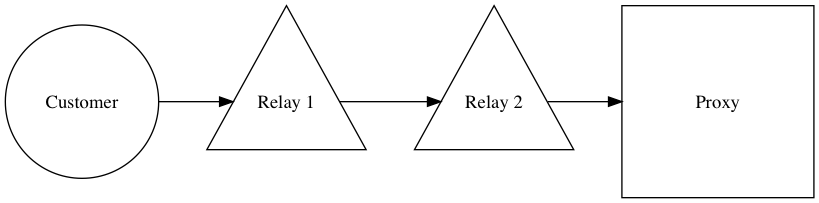
\includegraphics[width = 300pt]{sttc}
  \caption{A three-Econ Manifold routing traffic for a Customer}
\end{figure}

In this section we will describe the specification for Relay and Proxy
behavior, and discuss the ``chaining together'' of these nodes to
support uncensorable, anonymous web browsing.

\subsection{Specification for the Sale of Bandwidth}

Relay nodes implement a relatively simple behavior pattern:

\begin{itemize}
\item Maintain one or more connections, each with their own encryption key.
\item Check any tickets received, and cash-in winners.
\item Monitor the balance of trade, and disconnect if it exceeds a
  predeclared amount.
\item Receive data from any open connection, and perform decryption at
  message boundaries.
\item Process decrypted messages as follows:
  \begin{itemize}
  \item Forward any non-control segments to the connection(s)
    specified in the message.
  \item Process any control segments:
    \begin{itemize}
    \item \emph{Dummy Data.} Instructs the Relay to discard this segment.
    \item \emph{Burn at Rate.} Instructs the Relay to send data over a
      connection at a fixed rate, queueing packets and generating data
      as necessary to maintain the rate.
    \item \emph{Ratchet Ticket.} Instructs the Relay to pass a Ticket to
      the peer it received this packet from.
    \item \emph{Initiate Connection.} Instructs the Relay to establish a
      new connection. Used during setup and to handle disconnection.
    \item \emph{Initial Web Connection.} (Proxies Only.) Instructs the
      proxy to open an SSL connection to the specified host. To
      support whitelists, this cannot be a raw IP address.
    \end{itemize}
  \end{itemize}
\end{itemize}

%% [saurik: should we flesh out the above with packet specifics? I feel
%%   like *this* part of the document can/should be more specific than
%%   the rest, as we'd like transient nodes to be written more rapidly
%%   than full clients? Just a guess. - dls]

An important consideration in the above behavior is that no
proof-of-work is required of Relays on an ongoing basis. When combined
with all our connections being WebRTC connections, this leaves the
door open for websites potentially monetizing their visitors by
running pure javascript relay code.

For discussion of possible extensions via application specific control
segments, see Section \ref{sec:future}.

\subsection{Guard Nodes and ``Bandwidth Burning''}
\label{bandwidth-burning}

The relay that a customer is connected to has a very important piece
of information: the customer’s IP address. We assume customers will
want to keep this as private as possible, and so the default client
expresses a preference for long-lived peers as the first
hop.

Another concern for nodes at the first hop, which is discussed in
depth in our discussion of informational attacks stemming from
collusion (Section \ref{sec:collusion}), is they sit in an ideal
position to perform timing attacks. To prevent these attacks, we
recommend that privacy-conscious users employ a method called
\emph{Bandwidth Burning} -- paying the second hop to send a fixed
amount of bandwidth to the customer. As this approach results in
data-usage which is completely uncorrelated to network usage, this
approach prevents timing attacks performed by adversaries which cannot
see the inbound traffic of relay three.

To provide assistance to users seeking evasion (Section
\ref{sec:evasion}), bandwidth burning will also support non-fixed
rates determined by the statistical properties of popular non-\Orchid
WebRTC protocols.

\subsection{Chaining}

Customers interested in employing Relays for anonymous Internet
access, will use the above specification to create ``chains'' of
relays.



\section{Collusion Attacks on Manifolds}
\label{sec:collusion-attacks}
%%% collusion-attacks.tex: -*- LaTeX -*-  DESCRIPTIVE TEXT.
%%%
%%% Copyright (c) 2017 Brian J. Fox & Orchid Labs, Inc.
%%% Author: Brian J. Fox (bfox@meshlabs.org)
%%% Author: A truckload of others
%%% Birthdate: Tue Oct 10 12:04:54 2017.

%% Tasks for DLS:
%%
%% Nice to have:
%%   - sum of risk across all possible attacks for a given manifold length.

In this section we explore what kinds of information may be inferred
or deduced by an attacker controlling or monitoring multiple relays
and/or Internet Service Providers (ISPs). Using the assumption that
Relays and Proxies are selected randomly (and consequently so were
ISPs), we build a probability model of the chance that a given attack
may be performed at different manifold lengths.

\subsection{Information Available to Individual Relays and Proxys}
\label{relay-proxy-info-known}

Due to the inherent structure of IP-based networking, and the
\Orchid{} protocol's use of Ethereum based payments, Relay and Proxy
nodes \emph{and their IPSs} gain access to the following information:

\begin{itemize}
\item The IP addresses of all computers they are connected to.
\item The size, timing, and number of packets they forward.
\item The public key which controls the tokens paying them.
\item The contents of any control segments directed to them.
\end{itemize}

Additionally, Proxy nodes \emph{and their ISPs} gain access to the
following information:

\begin{itemize}
\item The hostname of the webserver, and the plantext portions of the
  SSL/TLS session negotiation.
\end{itemize}

\subsection{Potential Parties to a Collusion}
\label{sec:collusion}

The following roles have access to customer information, and so might
meaningfully collude or be monitored as part of an attack:

\begin{itemize}
\item The Internet Service Provider (ISP) of a customer, relay, proxy,
  or webserver. Untrustworthy with probability $s$.
\item Website. The webserver the proxy is connected to. Untrustworthy
  with probability $w$.
\item Relay$_n$. The nth relay in the chain. Untrustworthy with
  probability $\frac{r}{n}$.
\item Proxy. The proxy relaying bandwidth to the
  webserver. Untrustworthy with probability $\frac{x}{n}$.
\end{itemize}

We have separated out $r$ and $x$ above because although an attacker
cannot control the total amount of computation they have available for
proof-of-work computations, they can control how that computation is
allocated between relay and proxy nodes.

\subsection{Types of Attack}

The central goal of collusion attacks is the linking of a specific
\Orchid{} customer with a specific SSL connection. There are two ways
this can be done:

\begin{itemize}
\item Relation. When this is possible, the attacker can deduce that a
  customer is talking to a given website because they can observe
  enough points along the route.
\item Timing. When this is possible, the attacker can infer that a
  customer is talking to a given website by controlling and then
  observing the timing of packets.
\item Unburning. When this is possible, the attacker can perform a
  timing attack in spite of bandwidth burning being employed by the
  customer.
\end{itemize}

\subsection{``Regular'' Internet Access: Zero Relays, Zero Proxies}

Although the \Orchid{} system is of course not used when a Customer
directly connects to a website, we feel it is important to review what
informational risk are present in this setup to ground the rest of our
analysis.

\begin{center}
\begin{tabular}{l | l | l | l | l}
  ISP & Website & P(Relate)          & P(Timing)  & P(Unburn) \\
  \hline
  x   &         & $s$                & & \\
  \hline
      & x       & $w$                & & \\
\end{tabular}
\end{center}

In the above table, an ``X'' indicates participation in a collusion,
and the values in P(Relate) and P(Timing) indicates the chance of this
happening. Lines where attacks are not possible are omitted, as are
lines with extraneous ``X''s, and mention of more sophisticated
attacks where simpler attacks are possible.

\subsection{VPN: Zero Relays, Zero Proxies}

For the purposes of grounding our analysis, we also present the
collusion risk inherent to VPN access.

\begin{center}
\begin{tabular}{l | l | l | l | l | l}
  ISP & VPN & Website & P(Relate)          & P(Timing) & P(Unburn) \\
  \hline
      & x   &         & $g$                & & \\
  \hline
  x   &     & x       & $sw$               & & \\
\end{tabular}
\end{center}

Where $g$ is the chance the VPN provider is being monitored, or is
colluding with an adversary. Note that $g$ may change over time in
difficult to model ways, for example as a result of your VPN usage.

\subsection{Zero Relays, One Proxy}

%% \begin{figure}[htbp]
%%   \centering
%%   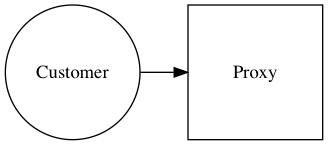
\includegraphics[width = 200pt]{sc}
%%   \caption{}
%% \end{figure}

\begin{center}
\begin{tabular}{l | l | l | l | l | l}
  ISP & Proxy & Website & P(Relate)          & P(Timing) & P(Unburn) \\
  \hline
      & x     &         & $\frac{x}{n}$      & & \\
  \hline
  x   &       & x       & $sw$               & & \\
\end{tabular}
\end{center}

It should come as no surprise that the risks in this case are quite
similar to those inherent to VPN usage. A manifold employing no relays
is equivalent to a VPN in which a new VPN provider is selected at
random before each browsing session, and no personal information is
stored by the VPN provider.

\subsection{One Relay, One Proxy}

%% \begin{figure}[htbp]
%%   \centering
%%   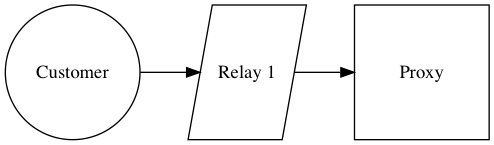
\includegraphics[width = 200pt]{stc}
%%   \caption{}
%% \end{figure}

\begin{center}
\begin{tabular}{l | l | l | l | l | l | l}
  ISP & Relay$_1$ & Proxy & Website & P(Relate)          & P(Timing) & P(Unburn) \\
  \hline
      & x         & x     &         & $(\frac{rx}{n^2})$ & & \\
  \hline
      & x         &       & x       & $w(\frac{r}{n})$   & & \\
  \hline
  x   &           & x     &         & $s(\frac{x}{n})$   & & \\
  \hline
  x   &           &       & x       &                    & $sw$ & \\
\end{tabular}
\end{center}

If bandwidth burning is employed in this configuration, all timing
attacks are mitigated. Observe that adding Relay$_1$ or the Proxy to
the Timing case allows for a Relation.

\subsection{Two Relays, One Proxy}

%% \begin{figure}[htbp]
%%   \centering
%%   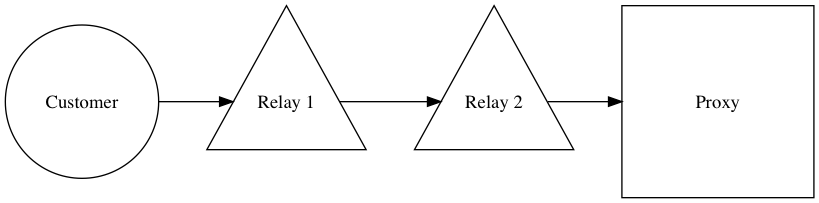
\includegraphics[width = 200pt]{sttc}
%%   \caption{}
%% \end{figure}

\begin{center}
\begin{tabular}{l | l | l | l | l | l | l | l}
  ISP & Relay$_1$ & Relay$_2$ & Proxy & Website & P(Relate)           & P(Timing) & P(Unburn) \\
  \hline
      & x         &           & x     &         & $(\frac{rx}{n^2})$  &           & \\
  \hline
  x   &           & x         & x     &         & $s(\frac{rx}{n^2})$ &           & \\
  \hline
      & x         & x         &       & x       & $w(\frac{r}{n})^2$  &           & \\
  \hline
  x   &           & x         &       & x       & $sw(\frac{r}{n})$   &           & \\
  \hline
      & x         &           &       & x       &                     & $s(\frac{r}{n})$ & \\
  \hline
  x   &           &           &       & x       &                     & $sw$      & \\
\end{tabular}
\end{center}

If bandwidth burning is employed in this configuration, all timing
attacks are mitigated. In the case of a timing attack carried out by
Relay$_1$ and the Website, adding Relay$_2$ or the Proxy to the
collusion results in a relation. In the case of the customer's ISP
colluding with the Website, adding Relay$_2$ results in a relation.

\subsection{Three Relays, One Proxy}

%% \begin{figure}[htbp]
%%   \centering
%%   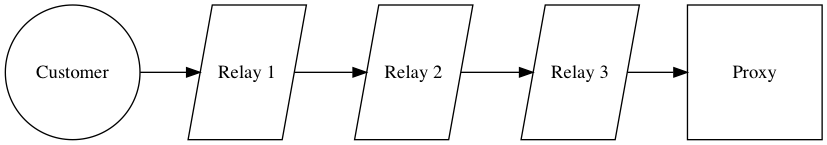
\includegraphics[width = 200pt]{stttc}
%%   \caption{}
%% \end{figure}

\begin{center}
\begin{tabular}{l | l | l | l | l | l | l | l | l}
  ISP & Relay$_1$ & Relay$_2$ & Relay$_3$ & Proxy & Website & P(Relate)             & P(Timing) & P(Unburn) \\
  \hline
      & x         & x         &           & x     &         & $(\frac{r^2x}{n^3})$  & & \\
  \hline
      & x         &           & x         & x     &         & $(\frac{r^2x}{n^3})$  & & \\
  \hline
  x   &           & x         &           & x     &         & $s(\frac{rx}{n^2})$ & & \\
  \hline
      & x         &           & x         &       & x       & $w(\frac{r}{n})^2$ & & \\
  \hline
  x   &           & x         & x         &       & x       & $sw(\frac{r}{n})^2$ & & \\
  \hline
      & x         &           &           &       & x       &                    & $s(\frac{r}{n})$ & \\
  \hline
  x   &           &           &           &       & x       &                    & $sw$ & \\
  \hline
      & x         & x         &           &       & x       &                    &      & $s(\frac{r}{n})^2$ \\
  \hline
  x   &           & x         &           &       & x       &                    &      & $sw(\frac{r}{n})$ \\
\end{tabular}
\end{center}


\section{SSL and TLS Vulnerabilities}
%%% ssl-vulnerabilities.tex: -*- LaTeX -*-  DESCRIPTIVE TEXT.
%%% 
%%% Copyright (c) 2017 Brian J. Fox & Orchid Labs, Inc.
%%% Author: Brian J. Fox (bfox@meshlabs.org)
%%% Author: A truckload of others
%%% Birthdate: Tue Oct 10 12:05:37 2017.

SSL and TLS are complicated protocols, receiving a constant stream of
security updates as implementation flaws are discovered.
Unfortunately, users sometimes delay upgrading their software, use
untrustworthy or poorly written software, and misconfigure their
software. To protect users as possible, the \Orchid{} Protocol provides
``sanity check'' features.

\subsubsection*{SSL Downgrade Attacks}

In so-called \emph{SSL Downgrade Attacks}, the attacker causes a
secure connection to use poor quality encryption
(\cite{ssl-downgrade}). To perform this attack, the attacker simply
removes mention of more secure encryption methods supported by the
client from the initial key negotiation packets. To prevent this
attack, the \Orchid{} Client automatically does the inverse where
possible -- it removes mention of insecure options from the key
negotiation packet (an ``SSL upgrade'' attack.)

\subsubsection*{Old Browsers and Phone Apps}

SSL and TLS security vulnerabilities are periodically found and
patched in web browsers. However, not all users can be assumed to use
up-to-date browsers. A similar situation occurs with mobile phone
apps, where developers sometimes omit things like SSL certificate
validation.

To address these issues, the \Orchid{} Client automatically verifies
certificate chains using an up-to-date copy of ``Boring SSL'' -- the
open source SSL library used in Google Chrome.

%% TODO: we need to flesh this out once we have an SSL expert on hand.

%% \subsection{Mitigation of 8.1.1 and 8.1.2}

%% \begin{enumerate}
%% \item Check SSL Certificates
%% \item Check SSL Versions, Cipher Suites
%% \item Check Basic Constraints
%% \item “Boring SSL”
%% \end{enumerate}




\section{The Agora}
\label{sec:agora}
%%% agora.tex: -*- LaTeX -*-  DESCRIPTIVE TEXT.
%%% 
%%% Copyright (c) 2017 Brian J. Fox & Orchid Labs, Inc.
%%% Author: Brian J. Fox (bfox@meshlabs.org)
%%% Author: A truckload of others
%%% Birthdate: Tue Oct 10 12:06:22 2017.

The Agora, named after the greek work for market, is a P2P network
similar in structure to a Distributed Hash Table (DHT), which serves
as a meeting ground for buyers and sellers of bandwidth.

\subsection{Fundamental Agora Operations}

At a high-level, the operations provided by the Agora are:

\begin{itemize}
\item A method for Econs to join the Agora.
\item A method for asking Econs what services they have for sale.
\item A method for selecting a subset of all peers, randomly weighted by computational resources, such that the \emph{lookup property} holds: $$lookup(rand(address)) \approx rand(Econ)$$
\end{itemize}

The \emph{lookup property} is important because it allows customers to
know with assurance that their chosen Econ is an attacker with
probability $\frac{a}{n}$.

To implement these operations, the Agora takes the structure of a DHT
with no keys and values. To perform the random selection, a user
simply generates a random address and locates the Econ closest to that
point.

\subsection{Fundamental Econ Operations}

The operations supported by Econs on the Agora are:

\begin{itemize}
\item \emph{Get Routing Table and Medallion}. This returns the Econ's proof of work and signed routing table for inspection, along with the cost of relaying traffic to members of the routing table.
\item \emph{Relay Traffic}. Pays the Econ to forward traffic to one of the peers in its routing table.
\item \emph{List Services}. Asks the Econ for a list of services it sells.
\item \emph{Purchase Service}. Employ the Econ as a service provider.
\end{itemize}

The first two of these are used by customers to navigate to an Econ of
interest, while the second two are used to negotiate the purchase of
services once that Econ is found.

Navigation through the Agora takes a form similar to that used in
Manifolds. A customer connects to some known Econ (found through
bootstrapping, see \ref{bootstrapping}), inspects its routing table,
and pays to forward traffic to the Econ closest to its chosen
point. As we will see in the section on routing tables, this allows
customers to keep their IP addresses secret, while still providing
relatively efficient random access to Econs of $O(log^2 n)$ packets.

\subsection{Chord Routing Structure}

[need graphic]

Econs are connected in the \Orchid{} Protocol using the same scheme used
in the Chord DHT.

Addresses are viewed as a ring of size $2^{256}$, and the distance
between peers at addresses $a, b \in [0, 2^{256}-1]$ is defined to be
$n$ s.t. $0 \leq n < 2^{256}$ and $a + n \equiv b \pmod{2^{256}}$.

For a collection of Econs in an Agora, $A$, the forced connections for
a given Econ $e$ are defined to be $\min_{f \in A} dist(e+t, f)$, for
each of 256 target addresses $t \in \{1, 2, 4, .. 2^{255}\}$.

We chose to use this routing structure because of its maturity,
successful track record in deployed systems, and correctness
proofs. Readers interested in learning more are encouraged to
read\cite{CHORD}. For our purposes, it is enough to note that the
following two properties are provided by this routing scheme:

\begin{enumerate}
\item \emph{Finite, Deterministic Connections}. Every Econ has a
  number of forced connections $\leq 256$.
\item \emph{Logarithmic Traversal Distance}. Given a random address
  $t$ and a random connected Econ $e$ with connections $C$, that
  $distance(e, t) \approx 2 * \min_{f \in C} distance(f, t)$. Because
  the distance will half with each hop, the expected traversal length
  on the network is $log_2(n)$ where $n$ is the network size.
\end{enumerate}

\subsection{Medallions on the Agora}

To prevent attackers from choosing their location on the Agora, the
location of Econs is defined to be the hash of their Medallion.  To
prevent an attacker from running more Econs than is proportional to
their share of the Agora's total computational power, every Econ
checks the validity of all its connections' Medallions every Medallion
cycle. In the event that a valid Medallion is not supplied, it is
disconnected from the network.

\subsection{Signed Routing and Eclipse Attacks}

%% In a fully distributed system, no one (except, perhaps, an attacker)
%% has a global view of the network. Attackers often seek to exploit this
%% by choosing to omit mention of options they do not wish others to use.

%% For example, imagine if in the above routing scheme an attacker chose
%% to lie about what connections it has – if the buyer has no way of
%% detecting this, they might be led off to a fake Agora in which all
%% ``participants'' were owned by the attacker. To put a stop to this
%% situation, Agora's routing tables are verified non-malicious by the
%% peers contained on them via an inductive proof.

%% To do this, an Econ joining the network first computes its forced
%% connections list $C$, then demonstrates to each $c \in C$ that (1)
%% every connection in $C$ is indeed forced, and (2) it is possible to
%% route from every element of $C$ to every other element. It does this
%% by supplying the chain of signed routing tables that led it to each
%% element of $C$.

%% Once the proof has been sent




%% When a node would like to establish a forced connection, that node
%% must first prove to each node on its forced connections list that each
%% other node on that list is a member of the same Agora. To do this, we
%% show them a chain of routing tables that connects them.


One of the issues that arises in distributed networks is that no one (except, perhaps, an attacker) has a global view of the network. For example, imagine if in the above routing scheme an attacker chose to lie about what connections it has – if the buyer has no way of detecting this, they might be led off to a fake Agora in which all “participants” were owned by the attacker. To put a stop to this situation, Agora's routing tables are verified non-malicious by the peers contained on them.

When a node would like to establish a forced connection, that node must prove to each node on its forced connections list that each other node on that list is a member of the same Agora. To do this, we first select a random econ $G$ by finding the Econ with an address closest to the hash of all the connections in the routing table $H(C_i)$. Then we supply:

\begin{enumerate}
\item Proof that all the Econs on the list can all route to $G$.
\item Proof that $G$ can route to each Econ
\item Proof that each Econ on the list is indeed a forced connection.
\end{enumerate}

These proofs all take the form of signed routing table chains which lead from $C_i$ to $G$, or in the case of (3) the chain of signed routing tables which led from the Entry Econ to each $C_i$. Once such proof has been provided, all of the peers on the new routing table sign the table, and the connecting Econ signs theirs. For those elements of $C_i$ for whom the new Econ is a forced connection, the same proof is sent to each of their connections for signature.

Because this is the only method for adding Econs to the Agora, these requirements form an inductive proof of the Agora's soundness. If one of the nodes in $C_i$ attempts to supply a fake routing table, it will not route to the same $G$ as the other Econs in $C_i$. If one of the nodes $C_i$ is not a member of the Agora, $G$ will not be able to route to them. If the Econ seeking to connect has lied about $C_i$ being nearest nodes to his forced connection points, (3) will demonstrate that to be false.

From these properties, we can see that the avenues left for an attacker are:

\begin{itemize}
\item If an attacker can generate a Medallion address such that all $C_i$ are controlled by them, the above system will cease to function. This will happen with probability $(\frac{a}{n})^{log(n)}$. If such a collision occurs, $(1 - \frac{n-log(n)}{n})^{log(n)}$ percent of all queries will be compromised. To put these numbers in perspective, if an attacker controls 10\% of the network, at 1 million nodes there is a 1e-8\% chance of such a collision happening, and if it does occur around 1e3\% of all system queries will be impacted. At 100 million nodes the chance drops to 1e-12\%, causing disruption of 1e-5\% of queries. Note this damage is repaired during Agora Regeneration \ref{agora-regen}.
\item If an attacker has now joined the network, but was forced to use a valid routing table, the only attacks it can perform are related to selling services, not routing traffic on the Agora. As this is the situation expected in the rest of our attack models (that an attacker will control a number of econs proportional to the computational resources), we do not consider this an attack.
\end{itemize}

\subsection{Eclipse Attacks and Regeneration}
\label{agora-regen}

Long lived P2P networks suffer from Eclipse attacks. Although the
above signed routing scheme can make these arbitrarily difficult by
involving ever increasing number of peers for verification, another
approach is simply to limit the lifespan of peers. For this reason,
Econs on the Agora must change keys every 100 Ethereum blocks.

%% This is ensured by $XOR(address, Eth)$

%% [Todo: finalize randomization schedule here.]

\subsection{Finding Entry Nodes}
\label{bootstrapping}

The distribution of Entry Nodes is a difficult topic. If oppressive governments are able to access this list, they will block user's abilities to access the list. We have therefore located essential services that would be internet-breaking if they were blocked, and have devised methods for adding Entry Node information to the data contained in them.

\subsection{Identifying \emph{the} Agora}

The above discussion discussion of security is ultimately meaningless if there is no way to locate ``the right Agora'' on a fresh machine. Any distribution method which exists for \emph{Entry Econs} can not be presumed immune from infiltration by fake Entry Nodes. To do so, we simply estimate the computing power of a given Agora, and select the right one. This is justified by our core security assumptions (Section \ref{core-security}).

\begin{itemize}
\item Density Estimation. Because an Econ's forced connections are defined to be the econs nearest to some set of points in a $2^{256}$ address space, in any real-world situation there will be measurable gaps between the ideal connections and the actual ones. To estimate density in this space, we can observe that these connections as the result of a random binomial process: every point between the ideal point and the actual point is a failure, and the actual point is a success. Therefore, for a given number of missing nodes $M$ and a given number of realized connections $C$, The uniform prior MAP estimate of network density is $$\frac{C}{C + M} 2^{256}$$.
\item Traversal Distance. The Agora provides address look ups in $O(log_2(n))$ hops. We can use this in reverse to estimate network density.
\end{itemize}

One might be inclined to believe that density estimation is enough, however a clever attacker in possession of a sybil network of modest size, will have free choice for which node is to be put forward as the the Entry Econs for the false network, while the Entry Econs from the ``real Agora'' will have a density which is a random sample from the network. To make matters worse, if the traversal distance is chosen as the metric, one might imagine an attacker who anticipates this, and so creates sub-optimal routing tables which require longer than the $O(log_2(n))$ to traverse. Thankfully, sub-optimally connected Agoras will perform worse on the density metric. The verification method used in the \Orchid{} System is to traverse to a random address, saving the routing tables along the way, and then perform a density estimate using the routing table from all but the first two hops.

%% \subsection{Economics}

%% \subsubsection{Price Discovery}

%% Uers may set their own price for bandwidth, but this is hardly
%% satisfying. Some users may price themselves out of the market, and
%% other users may charge too little. We therefore provide the following
%% algorithm for users who wish to maximize their profit as bandwidth
%% sellers:

%% \begin{algorithm}[H]
%%   \KwData{Quantity of bandwidth the user wishes to sell, $Q$}
%%   \KwData{Amount of data sold in the last 10 minutes, $S_t$}
%%   \KwData{Price of the previous data sold, $P_t$}
%%   \KwResult{A New Price $P_{t+1}$}
%%   \While{$S_t > Q$}{
%%     return $S_t$ * 1.1;
%%   }
%%   return $(S_t - Q) * 0.01 * P_t$ ;
%%   \caption{Automatic Price Scaling}
%% \end{algorithm}

%% \subsubsection{Auction Design}

\subsection{Proxy Whitelists}

Some users wishing to offer Proxy services may not be comfortable offering ``open access''. For example, allowing users to access facebook.com has a risk profile similar to acting as a relay, while allowing arbitrary connections to the internet may result in a visit from local law enforcement. Econs on the Agora may therefore set a whilelist of websites they will allow users to contact when using them as a Proxy, and specify their whitelists in their responses to \emph{Get Offers}.


%% TODO tonight?
%% \section{Economic Soundness}
%% \label{sec:economic-soundness}

\section{Firewall Circumvention Features}
\label{sec:evasion}
%%% firewall.tex: -*- LaTeX -*-  DESCRIPTIVE TEXT.
%%%
%%% Copyright (c) 2017 Brian J. Fox & Orchid Labs, Inc.
%%% Author: Brian J. Fox (bfox@meshlabs.org)
%%% Author: A truckload of others
%%% Birthdate: Tue Oct 10 12:07:15 2017.

The above system would be of little use if only users already
possessing free and open access to the Internet could use it. In this
section we will discuss features which ease access for those users
whose Internet access is provided by their attacker.

Please note that if an adversary is willing to completely block all
Internet access, no defense in this area is possible. All defense
analysis in this section therefore assumes that the attacker suffers
some cost for blanket blocking, and seeks to maximize this cost in the
hope that sufficiently costly attacks will not be performed.

\subsection{Bootstrapping}

One of the first attacks we anticipate firewall providers to attempt
against the \Orchid{} Network is to create a list of Entry Peddlers, and to
block all access to them. This is because if customers can not access
Entry Peddlers, they could not use the network. Complicating matters, a
competent attacker must be assumed to have any list of IP addresses
available to customers.

%% To address this initially, we will provide a service which allows
%% users to perform a ``group buy'' of a small VPS instance to act as a
%% relay in exchange for tokens. Customers would then use this relay as a
%% mechanism for accessing the rest of the network, making the security
%% analysis identical to that in Section \ref{sec:collision}, with Orchid
%% Labs also acting as a secondary ISP. Since this VPS's IP address is
%% drawn from IP addresses used to host websites generally, we anticipate
%% that blanket blocking of these IP addresses would be quite costly.

To address this initially, we will provide a service which allows
users to learn fresh Relay IP addresses in exchange for proof-of-work.
To hinder blocking of the bootstrapping back and forth itself, we will
provide access to this boostrapping service via web, email, and
popular instant messaging platforms. The user will copy/paste a
challenge from their client's options screen into the most convenient
communications mechanism, then copy/paste the reply back into the
client.

\subsection{DPI, Inference, and Active Probing}

More sophisticated firewalls employ methods such as Deep Packet
Inspection (DPI; analysis of the contents of packets rather than just
the headers), timing inference (the use of aggregate statistical
measures over packet size, quantity, and timing), as well as active
probing (attempting connection with the user or the server they are
connecting to in an attempt to identify the service being provided.)

We do not anticipate the use of deep packet inspection or active
probing to provide significant information. Through our use of WebRTC,
all communication is encrypted and there are no open ports unless an
active WebRTC offer has been issued. Since this matches the behavior
of all other uses of WebRTC, this behavior can not disambiguate \Orchid{}
users.

Timing inference is potentially an effective method for detecting
\Orchid{} users, as the timing and size of web requests over an encrypted
stream are unlikely to look like other kinds of WebRTC traffic
(\cite{peekaboo}). To address this, users accessing the \Orchid{} Network
in situations where inference attacks are likely are encouraged to use
``bandwidth burning'' (Section \ref{bandwidth-burning}).

\subsection{Disclosure: Ethereum Traffic}

Because the current client employs an Ethereum client to track payment
statuses, and Ethereum has its own non-hardened networking signature,
detection related to this Ethereum traffic is likely to be the weak
link. Firewall operators may simply ask ``is the computer running
Ethereum \emph{and} consuming large amounts of WebRTC traffic?''

To maintain project focus, hardening of Ethereum and/or serving
Ethereum traffic over the \Orchid{} Network is not a feature of our
initial release. We plan on addressing this in future versions, see
Section \ref{securing-eth}.


\section{Current State of the Software}
\label{sec:current}
%%% software-status.tex: -*- LaTeX -*-  DESCRIPTIVE TEXT.
%%% 
%%% Copyright (c) 2017 Brian J. Fox & Orchid Labs, Inc.
%%% Author: Brian J. Fox (bfox@meshlabs.org)
%%% Author: A truckload of others
%%% Birthdate: Tue Oct 10 12:07:47 2017.

[Note the software is being actively developed right now. The
  following describes where we hope to be when we publicly release
  this whitepaper. Current, and potentially obsolete comments are in
  brackets.]

\subsection{Software for the Ethereum Platform}

We have a ERC20 compliant token, a smart-contract implementing
stochastic micropayments as described in Section \ref{sec:tickets},
including javascript helper functions for the creation, validation,
and claiming of ticket winnings. Readers interested in viewing or
auditing the code are invited to visit [TODO: public github link.]

[Initial implementation here is complete. We are beginning the
  security audits of this, and polishing while we wait.]

\subsection{Core Networking Client}

We have completed an initial implementation of the proceeding protocol
in Microsoft's TypeScript (a statically typed variant of the
javascript language which compiles to javascript.) Readers interested
in auditing the code are invited to view it at [TODO: public github link.]

[Initial implementation is ongoing, and may lead to minor changes to
  this document. After the software is complete, the security audit
  will begin.]

\subsection{User Interface}

We have constructed a genuinely user-friendly interface to provide
users with minimal technical ability use of our Ethereum and Core
Networking software.

[Initial implementation is ongoing. Security audit will begin on
  completion, usability testing will start in earnest during our alpha
  release.]



\section{Performance Scaling}
\label{sec:performance}
%%% performance.tex: -*- LaTeX -*-  DESCRIPTIVE TEXT.
%%%
%%% Copyright (c) 2017 Brian J. Fox & Orchid Labs, Inc.
%%% Author: Brian J. Fox (bfox@meshlabs.org)
%%% Author: A truckload of others
%%% Birthdate: Tue Oct 10 12:08:14 2017.

In this section we examine how the system will function as the
number of users grows.

\subsection{Algorithmic Performance}

Broadly, there are three parts to the \Orchid{} Protocol: Ethereum-based
payments, manifolds, and \tOM{}.

Ethereum-based payments scale with Ethereum as normal transactions.
Having reviewed the Ethereum system design, we are confident that even
if the \Orchid{} Network is extremely successful, and becomes a
significant percentage of the Ethereum's total transaction volume,
this component will function within design tolerances.

Manifolds are chains of bandwidth sellers (Relays and Proxies)
all of which have performance characteristics independent of the total number of
\Orchid{} Network participants.

The core operations of \tOM{} are based on the well-studied Chord
DHT. The number of connections that Peddlers must maintain grows at a
rate of $O(log{}n)$, to a maximum of 256 connections. Queries on the
network require $O(log{}n)$ hops. Although these operations do become
more burdensome as the network increases in size, we do not believe
any significant impact on performance will result.

\subsection{Allocation of Scarce Resources}

The \Orchid{} Protocol is built around tokens. These tokens will allow,
through price discovery, for graceful handling of a change in balance
between buyers and sellers.

For example, if Relays are in short supply, rather than providing all
customers with a slow experience, customers will engage in a bidding
war to determine who can use the system until the shortage is
corrected. Conversely, if Relays are in abundant supply, some Relays
may leave the system until such time as prices rise.

\subsection{Real-World Performance}

As the software is not yet complete, we do not have concrete numbers
to provide here. On release we will update this document with the
following graphs:

\begin{enumerate}
\item Chain setup time as a function of Orchid Market size.
\item Orchid Market join time as a function of Orchid Market size.
\item How quickly the price adjusts to scarcity, abundance.
\item Add any interesting ideas here!
\end{enumerate}


\section{Attack Analysis and Attacker User Stories}
\label{sec:attack-stories}
%%% attack-analysis.tex: -*- LaTeX -*-  DESCRIPTIVE TEXT.
%%%
%%% Copyright (c) 2017 Brian J. Fox & Orchid Labs, Inc.
%%% Author: Brian J. Fox (bfox@meshlabs.org)
%%% Author: A truckload of others
%%% Birthdate: Tue Oct 10 12:08:49 2017.

\subsection{Oppressive Web Applications}

Attacker Goals: Identify all \Orchid{} Relay and Proxy IP addresses.

Because \tOM{} contains all Relays and Proxies, this is the inverse
attack of the one discussed in Section \ref{sec:evasion}.

The number of forced connections on \tOM{} grows at $O(log{} n)$ where
n is the network size. If an attacker holds $m\%$ of global
computation, they will learn $log(n)$ IP addresses each time they
complete a proof-of-work computation. In $c$ epochs they will
therefore learn $1 - (1 - \frac{log(n)}{n})^c$ percent of the Relay and
Proxy IP addresses.

Readers familiar with the how the blocking of Tor traffic panned out
may worry the above describes a dire issue for the system.
Fortunately, this is not the case. Tor has around 1,000 exit 
nodes, which allowed for easy filtering. In our case, largely due to
our support for whitelists, we expect to have hundreds of thousands of
exit nodes. In addition to this forming a much larger computational
challenge to unmask using the above method, blocking these IP
addresses would result in the oppressive Web Application blocking
their own users.

\subsection{Corporate Networks and ``Great'' Firewalls}

Attacker Goals: Prevent usage of the \Orchid{} network by users to whom
you provide Internet access.

Features related to this are discussed in more detail in Section
\ref{sec:evasion}. The outlook for this attacker is bleak: \Orchid{}
network usage presents as WebRTC connections relaying a fixed amount
of data. There are no open ports to probe, and no IP addresses which
can be relied on to ``out'' them.

\subsection{Passive Monitoring and Inference, perhaps with Sybil Attacks}

Attacker Goals: Learn Customer IP Identification, and Website Identification.

Analysis related to this class of attack are discussed in more detail
in Section \ref{sec:collusion}. The outlook for this attacker is
bleak: the difficulty of positioning yourself in several positions of
a Chain requires possessing (and dedicating to this attack) a large
percentage of global computation power.

\subsection{Small-Time Trolling and QoS Attacks}

Synopsis: An attacker would like to cause mayhem on as much of the network as possible.

Security minded readers looking for a good time are encouraged to
perform analysis in this domain. The task here is, given a limited
budget (perhaps on the order of \$10,000 USD), to disrupt the network
as much as possible.

\subsubsection{Attacking Chains}

Attackers may try a variety of attacks here: randomly dropping
packets, providing only very slow service, providing intermittently
slow service, or simply disconnecting. In all cases, the customer
simply replaces the node in question, leading to a minor inconvenience
spread across all customers. An additional inconvenience may be caused
to other relays in the case of dropping packets, since there may be no
way of determining if A did not forward the packet of if B is lying
about not having received it. In this case the customer replaces both
Relays.

\subsubsection{Attacking \tOM{}}

Attackers have similarly many options for this situation.

One option is to improperly implement the joining protocol. We do not
view this as an attack, as in this case our ``attacker'' is simply
paying other Econs for packet forwarding.

Another option is to join \tOM{} and refuse to provide routing table
information to users, or refuse to forward packets. This will result
in some additional routing burden on $\frac{log(n)}{n}$ of \tOM{}
queries until the Peddler in question is disconnected from the
network.

A third option is to sit on \tOM{} while offering no services. In this
case auctions performed by customers become less efficient (suffering
from the loss of one participant $\frac{log(n)}{n}$ of the time).


\section{Future Work}
\label{sec:future}
%%% future-work.tex: -*- LaTeX -*-  DESCRIPTIVE TEXT.
%%% 
%%% Copyright (c) 2017 Brian J. Fox & Orchid Labs, Inc.
%%% Author: Brian J. Fox (bfox@meshlabs.org)
%%% Author: A truckload of others
%%% Birthdate: Tue Oct 10 12:09:40 2017.

The items in this section fall into two categories: nice-to-haves, and features we are internally conflicted about releasing to the public. We believe this is conflictedness is universal -- although almost everyone has favorite examples of power being used for oppression, there are also countless examples of power being used for good. Protocols like \Orchid{} have no judgement of their own, and so cannot tell if they are routing traffic for a freedom fighter or a terrorist, villain or hero.

\subsection{Proof of Space}
\label{future:proof-of-space}

As mentioned in Section \ref{medallions}, we are very interested in
exploring alternative proof types. This is an important issue both
because of the environmental impact of proof-of-work systems, and
because our current proof-of-work algorithm requires full blown
computers to act as network routers.

We are excited to explore the possibility of using disk space to be
the scarce resource at the core of our security, which might allow old
phones or similar hardware to profitably participate in the \Orchid{}
network.

\subsection{Protecting Content Hosts}
\label{subsec:protocol-extentions}

Many prior approaches (Section \ref{sec:prior-work}) discovered that content hosts sought similar protections as web users. We are internally conflicted on this point, as we do believe there is content which it is in the public interest not to have freely distributed (information related to the manufacture of nuclear weapons for example). However, should unforseen circumstances demand it, \Orchid{} could be extended to support such ``unrestricted, unsurveilled Hosts'' as seen in the following diagram:

\begin{figure}[htbp]
  \centering
  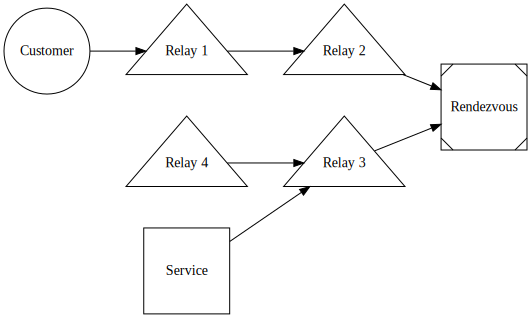
\includegraphics[width = 300pt]{sttRttc}
  \caption{A rendezvous node acting as a relay between a Service and a Customer}
\end{figure}

\subsection{Securing Ethereum Traffic}
\label{securing-eth}

As discussed in our section on firewall avoidance (Section \ref{sec:evasion}),
the Ethereum network traffic of clients is likely to be the weak
link. Because all nodes must maintain this information, use of the
\Orchid{} protocol to distribute Ethereum information seems like a
natural fit.

Unfortunately, relying on those you are paying for information about
payments leads to tricky issues. We hope to add this in the near
future, but will not be including it in our initial release.

\subsection{\Orchid{} as a Platform}

Although we anticipate that design of the core system will take up
much of our time for the immediate future, we are very interested in
the possibility that adding features to support the following use
cases may drastically increase the amount of bandwidth routed through
the \Orchid{} Network.

\begin{enumerate}
\item APIs for websites to directly interface to the network, and
  incorporate tokens into their service.
\item On-Network file storage and static website hosting.
\item File Sharing.
\item Email/Messaging service.
\item An arbitration/moderation service.
\end{enumerate}

%% The issue with modern networking from an surveillance perspective is that it is fundamentally about connections between computers. So long as the model is that a user's computer connects to a specific webserver to access a website, Orchid may be as good as possible. However, if we



%% \nocite{*}
\printbibliography

\end{document}
